\section{Angular dependency of the proton energy}

\section{Target dependency of the Rutherford cross section}

\section{Thickness of the target layers} 
Most of the particles pass directly through the target without scattering however a small amount gets scattered. When particles pass through the first layer the particles loose part of their energy, which means that the particles scattered on the second layer have lower energies when entering the second layer than if they had not passed through the first layer. By comparing measurements of scattering on the target with gold layer facing the beam and the carbon layer facing the beam, the distributions for scattering on carbon and gold are observed at different energies. 


\begin{figure}[h]
\centering
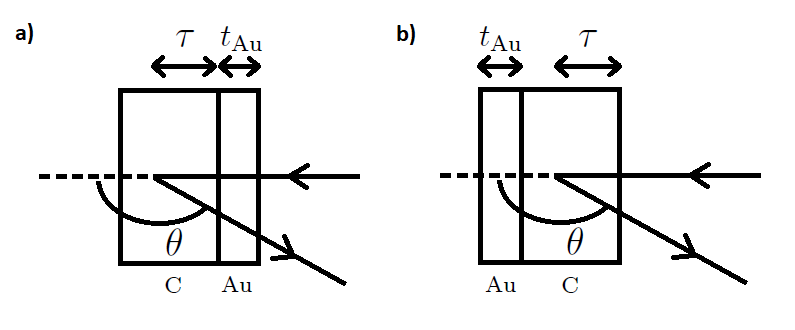
\includegraphics[width=0.99\columnwidth]{tykkelse.png}
\caption{Sketch of how to determine thickness of the target carbon layer from the energy difference between: a) gold layer facing the beam and b) carbon layer facing the beam.}
\label{fig_sketch_thickness}
\end{figure}


%The energies of the scattered protons is due to the ratio between the mass of the protons and the mass of the target. 
The changes in energies are proportional to the thickness of target layers. For the determination of the thickness of the carbon layer consider what happens to the energy in the two following situations. In situation a) gold is facing the beam, and the final energy is given as the incoming minus the energy lost due to scattering on gold:
\begin{equation*}
Ea_f = E_i (1-f(\theta)), 
\end{equation*}
where $f_{Au}(\theta)$ is the function giving the relation between the incoming energy $E_i$ and the particle energy $E_f$ in equation \cref{eq:5} after scattering on gold. 
In situation b) carbon is facing the beam, and the final energy is given as the incoming energy minus the energy lost due to the following: passing through the carbon layer, scattering on gold, and passing through the carbon layer again on the way out. 
\begin{align*}
Eb_f &= E_i - t_\mathrm{C} \left(\frac{dE}{dx}\right)_\mathrm{C} 
\\ &- f_\mathrm{Au}(\theta) \left(E_i - t_\mathrm{C} \left(\frac{dE}{dx}\right)_\mathrm{C} \right) \\ &- \frac{t_\mathrm{C}}{\cos(\pi-\theta)} \left(\frac{dE}{dx}\right)_\mathrm{C}, 
\end{align*}
where $\left(\frac{dE}{dx}\right)_\mathrm{C}$ is the stopping power of carbon found in the table in the laboratory.

The energy change for the peak position of the distribution for gold is found as the difference between the two situations. Thus, the thickness of the carbon layer is found as 
\begin{equation}
t_\mathrm{C} = \frac{\Delta E_{\mathrm{Au}}}{\left(\frac{dE}{dx}\right)_\mathrm{C} \left(1 - f_\mathrm{Au}(\theta) - \frac{1}{\cos(\theta)} \right)}
\end{equation}



%The thickness of the gold layer is found using the same approach for gold.
%\begin{equation}
%\Delta E_{Au} = t_C \left(\frac{dE}{dx}\right)_C \left(1 - f_E(\theta) + %\frac{1}{\cos(\pi-\theta)} \right),
%\end{equation}



\begin{figure}[t]
\centering
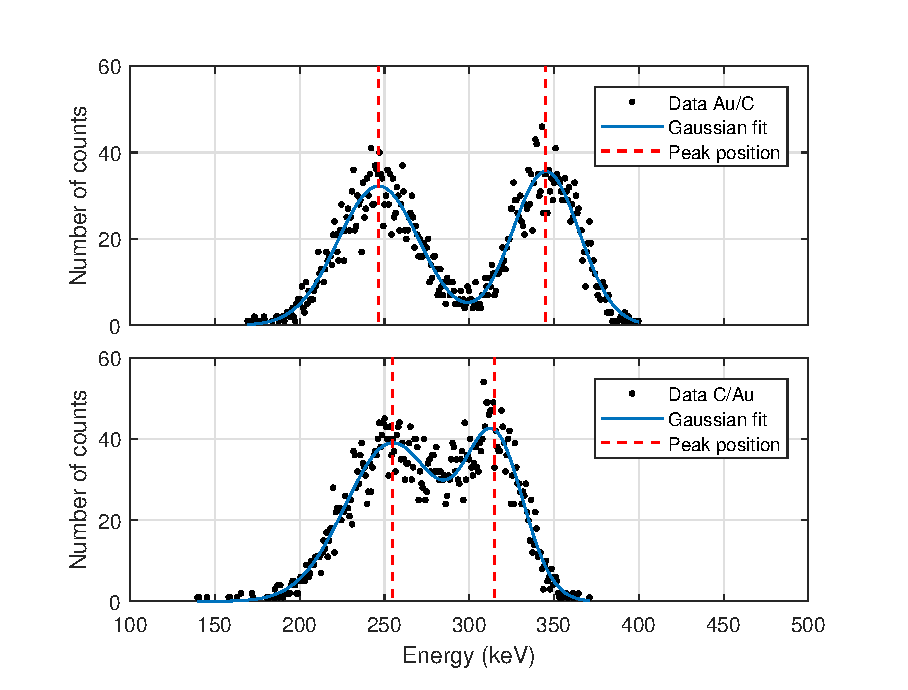
\includegraphics[width=0.99\columnwidth]{Dterminethicknessplot.eps}
\caption{Thickness of target layers determined from change in energy. Upper: gold layer facing the beam. Lower: carbon layer facing the beam.}
\label{fig_thickness}
\end{figure}



\section{Nuclear reactions of protons with boron}

